
%%%%%%%%%%%%%%%%%%%%%%%%%%%%%%%%%%%%%%%%%%%%%%%%%%%%%%%%%%%%%%%%%%%%%%%%%%%%%%%%%%%%%%%
%%%%%%%%%%%%%%%%%%%%%%%%%%%%%%%%%%%%%%%%%%%%%%%%%%%%%%%%%%%%%%%%%%%%%%%%%%%%%%%%%%%%%%%
% 
% This top part of the document is called the 'preamble'.  Modify it with caution!
%
% The real document starts below where it says 'The main document starts here'.

\documentclass[12pt]{article}

\usepackage{amssymb,amsmath,amsthm}
\usepackage[top=1in, bottom=1in, left=1.25in, right=1.25in]{geometry}
\usepackage{fancyhdr}
\usepackage{enumerate}
\usepackage{listings}
\usepackage{graphicx}
\usepackage{float}

\usepackage{mwe}
\usepackage{caption}
\usepackage{subcaption}
% Comment the following line to use TeX's default font of Computer Modern.
\usepackage{times,txfonts}



\makeatletter
\renewcommand*\env@matrix[1][*\c@MaxMatrixCols c]{%
  \hskip -\arraycolsep
  \let\@ifnextchar\new@ifnextchar
  \array{#1}}
\makeatother

\newtheoremstyle{homework}% name of the style to be used
  {18pt}% measure of space to leave above the theorem. E.g.: 3pt
  {12pt}% measure of space to leave below the theorem. E.g.: 3pt
  {}% name of font to use in the body of the theorem
  {}% measure of space to indent
  {\bfseries}% name of head font
  {:}% punctuation between head and body
  {2ex}% space after theorem head; " " = normal interword space
  {}% Manually specify head
\theoremstyle{homework} 

% Set up an Exercise environment and a Solution label.
\newtheorem*{exercisecore}{Exercise \@currentlabel}
\newenvironment{exercise}[1]
{\def\@currentlabel{#1}\exercisecore}
{\endexercisecore}

\newcommand{\localhead}[1]{\par\smallskip\noindent\textbf{#1}\nobreak\\}%
\newcommand\solution{\localhead{Solution:}}

%%%%%%%%%%%%%%%%%%%%%%%%%%%%%%%%%%%%%%%%%%%%%%%%%%%%%%%%%%%%%%%%%%%%%%%%
%
% Stuff for getting the name/document date/title across the header
\makeatletter
\RequirePackage{fancyhdr}
\pagestyle{fancy}
\fancyfoot[C]{\ifnum \value{page} > 1\relax\thepage\fi}
\fancyhead[L]{\ifx\@doclabel\@empty\else\@doclabel\fi}
\fancyhead[C]{\ifx\@docdate\@empty\else\@docdate\fi}
\fancyhead[R]{\ifx\@docauthor\@empty\else\@docauthor\fi}
\headheight 15pt

\def\doclabel#1{\gdef\@doclabel{#1}}
\doclabel{Use {\tt\textbackslash doclabel\{MY LABEL\}}.}
\def\docdate#1{\gdef\@docdate{#1}}
\docdate{Use {\tt\textbackslash docdate\{MY DATE\}}.}
\def\docauthor#1{\gdef\@docauthor{#1}}
\docauthor{Use {\tt\textbackslash docauthor\{MY NAME\}}.}
\makeatother

% Shortcuts for blackboard bold number sets (reals, integers, etc.)
\newcommand{\Reals}{\ensuremath{\mathbb R}}
\newcommand{\Nats}{\ensuremath{\mathbb N}}
\newcommand{\Ints}{\ensuremath{\mathbb Z}}
\newcommand{\Rats}{\ensuremath{\mathbb Q}}
\newcommand{\Cplx}{\ensuremath{\mathbb C}}
%% Some equivalents that some people may prefer.
\let\RR\Reals
\let\NN\Nats
\let\II\Ints
\let\CC\Cplx

%%%%%%%%%%%%%%%%%%%%%%%%%%%%%%%%%%%%%%%%%%%%%%%%%%%%%%%%%%%%%%%%%%%%%%%%%%%%%%%%%%%%%%%
%%%%%%%%%%%%%%%%%%%%%%%%%%%%%%%%%%%%%%%%%%%%%%%%%%%%%%%%%%%%%%%%%%%%%%%%%%%%%%%%%%%%%%%
% 
% The main document start here.

% The following commands set up the material that appears in the header.
\doclabel{STAT 401: Homework 5}
\docauthor{Stefano Fochesatto}
\docdate{\today}


%\begin{figure}[H]
%  \begin{center}
%  \caption{}
%  \includegraphics[\textwidth]{}
%  \end{center}
%\end{figure}

% \textbf{Code:}
% \begin{center}
% \lstinputlisting{}
% \end{center} 



\begin{document}

\begin{exercise}{1}Consider the national Football League data se named table.bu in the MPV package. 
  Use ?table.b1 to learn about its contents. Then do the following:

  \begin{enumerate}
    \item[a.] Fit a MLR model relating the number of games won to the team's passing yardage($x_2$),
    the percentage of rushing plays($x_7$), and the opponents yards rushing($x_8$). Calculate t-statistics for testing the hypothesis, 
    \begin{equation*}
      H_0: \beta_2 = 0
    \end{equation*} 
    \begin{equation*}
      H_0: \beta_7 = 0
    \end{equation*} 
    \begin{equation*}
      H_0: \beta_8 = 0
    \end{equation*} 
    \solution 
     \textbf{Code:}
     \begin{center}
     \lstinputlisting{r1.txt}
     \end{center} 
     \newpage

     \item[b.] Fit a $95\%$ confidence interval on $\beta_7$ and provide an interpretation of it. \\
    \solution From the given confidence interval we know that $95\%$ of the time the true value of $\beta_7$
    will be between $(0.011855322,0.376065098)$.\\
     \textbf{Code:}
     \begin{center}
     \lstinputlisting{r2.txt}
     \end{center} 
     \newpage

     \item[c.] Find a $95\%$ confidence interval on the mean number of games won by a team when $x_2 = 2300$,
     $x_7 = 56.0$, and $x_8 = 2100$.\\
     \solution
     \textbf{Code:}
     \begin{center}
     \lstinputlisting{r3.txt}
     \end{center} 
     \newpage

     \item[d.] Find a $95\%$ prediction interval on the mean number of games won by a team when $x_2 = 2300$,
     $x_7 = 56.0$, and $x_8 = 2100$.\\
     \solution
     \textbf{Code:}
     \begin{center}
     \lstinputlisting{r4.txt}
     \end{center} 
  \end{enumerate}
\end{exercise}





\newpage
 
\begin{exercise}{2} Data on last year's sales (y, in 100,000s of dollars) in 15 sales districts are give in the file 'sales'
  posted on Canvas. this file also contains promotion expenditures ($x_1$ in the thousands of dollars), the number 
  of active accounts $(x_2)$, the number of competing brands $(x_3)$ , and the district potential $(x_4)$ for each 
  of the districts.\\
  A model with all four regressors is proposed, 
  \begin{equation*}
    y = \beta_0 + \beta_1x_1 + \beta_2x_2 + \beta_3x_3 + \beta_4x_4 + e, e ~ N(0, \sigma^2)
  \end{equation*}
  Test the following hypothesis: 
  \begin{enumerate}
    \item[a.] $\beta_4 = 0$,
    \solution 
    Fitting the model and computing the test statistic we get the following, 
    \solution
    \textbf{Code:}
    \begin{center}
    \lstinputlisting[basicstyle = \small]{r5.txt}
    \end{center} 
    \newpage


    \item[b.]$\beta_2 = \beta_3 = 0$\\
    \solution For this hypothesis we will need to substitute our values for $\beta_2, \beta_3$ to create a new
    simpler model and compute the F statistic. By substitution our Null model looks like, 
    \begin{equation*}
      y_{null} = \beta_0 + \beta_1x_1 + \beta_4x_4 + e, e ~ N(0, \sigma^2).
    \end{equation*}
    Fitting the model, computing the F-statistic and p-value,\\ 
    \textbf{Code:}
    \begin{center}
    \lstinputlisting[basicstyle = \small]{r6.txt}
    \end{center} 
    \newpage


   \item[c.]$\beta_2 = \beta_3$\\
   \solution Again substituting $\beta_2 = \beta_3$ into our model to obtain a simplified model we get, 
   \begin{equation*}
    y_{null} = \beta_0 + \beta_1x_1 + \beta_2x_2 + \beta_2x_3+ \beta_4x_4 + e, e ~ N(0, \sigma^2).
  \end{equation*}
  \begin{equation*}
    y_{null} = \beta_0 + \beta_1x_1 + \beta_2(x_2 +x_3) + \beta_4x_4 + e, e ~ N(0, \sigma^2).
  \end{equation*}
  Fitting the model, computing the F-statistic and p-value, \\
   \textbf{Code:}
   \begin{center}
   \lstinputlisting[basicstyle = \small]{r7.txt}
   \end{center} 
   \newpage

   \item[d.] $\beta_1 = \beta_2 = \beta_3 = \beta_4 = 0$\\
   \solution Recall that the omnibus test is included in the model summary, looking at the 
   summary of our full model we get,   \\
   \textbf{Code:}
   \begin{center}
   \lstinputlisting[basicstyle = \small]{r8.txt}
   \end{center} 
   \newpage
  \end{enumerate}  
\end{exercise}



\begin{exercise} The variable $Y$ is believed to be associated with the variables $x_1, x_2, x_3,$ and $x_4$.
  All possible subsets of these variables are used in fitting a multiple linear regression model and the $RSS$ 
  and its df of the mode are recorded below, 
    \begin{figure}[H]
    \begin{center}
    \caption{MLR models, RSS, df}
    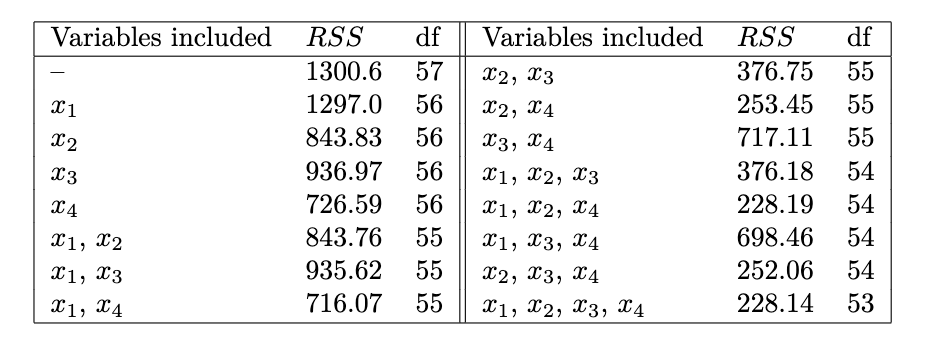
\includegraphics[width = \textwidth]{p1.png}
    \end{center}
    \end{figure}
  \begin{enumerate}
    \item[a.] Create an ANOVA table for the full linear model using Type I sums of squares. Include $F$ statistics 
    and p-values for testing individual predictors. \\

    \solution
    \begin{equation*}
      \begin{bmatrix}
        Source & SS & df & MS & F & p\\
        x_1 & 3.06 & 1
        x_2 & 453.24 & 1
        x_3 & 467.58 & 1
        x_4 & 148.04 & 1
        Error & 228.14 & 53
        Total & 1300.6 & 57

      \end{bmatrix}
    \end{equation*}
  \end{enumerate}


  
\end{exercise}



\end{document}





















